\documentclass[border=2mm,class=extreport,12pt]{standalone}

\usepackage{tikz}
\usetikzlibrary{arrows.meta,positioning}

\begin{document}
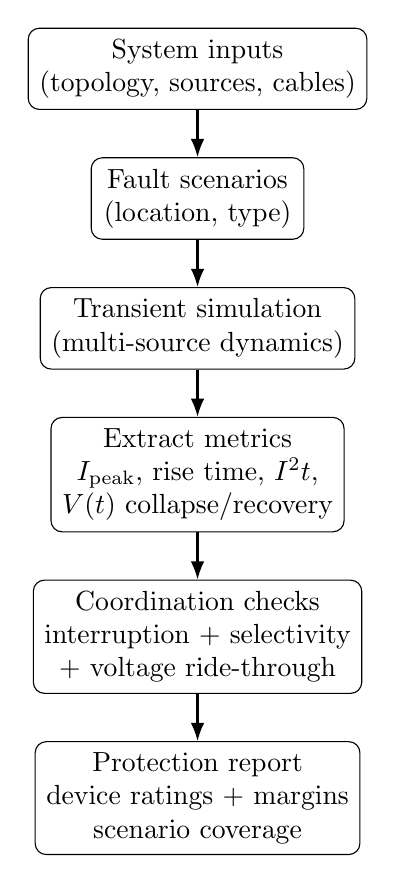
\begin{tikzpicture}[
    node distance=6mm and 10mm,
    box/.style={draw,rounded corners,align=center,inner sep=4pt,minimum width=2.7cm,minimum height=7mm},
    arrow/.style={-Latex,thick}
]

\node[box] (inputs) {System inputs\\(topology, sources, cables)};
\node[box,below=of inputs] (faults) {Fault scenarios\\(location, type)};
\node[box,below=of faults] (simulate) {Transient simulation\\(multi-source dynamics)};
\node[box,below=of simulate] (metrics) {Extract metrics\\$I_{\mathrm{peak}}$, rise time, $I^2t$,\\$V(t)$ collapse/recovery};
\node[box,below=of metrics] (coord) {Coordination checks\\interruption + selectivity\\+ voltage ride-through};
\node[box,below=of coord] (report) {Protection report\\device ratings + margins\\scenario coverage};

\draw[arrow] (inputs) -- (faults);
\draw[arrow] (faults) -- (simulate);
\draw[arrow] (simulate) -- (metrics);
\draw[arrow] (metrics) -- (coord);
\draw[arrow] (coord) -- (report);

\end{tikzpicture}
\end{document}
